\subsection{Sentence View}
\label{sec:sentence}
To start an exploration cycle, the experts need to examine the premise and hypothesis sentence the current example.
As illustrated in Fig.~\ref{fig:sentenceView}, the sentence view shows the premise and hypothesis sentence in (c) and (d).
%
To facilitate the analysis task (\textbf{T1}), we employ an automate sentence perturbation scheme that replaces nous and verb by their synonymous in the wordNet~\cite{Miller1995} (the standard lexical database for NLP applications).
%
When perturbation is applied to either of the sentences, the replaced words are highlight in blue (see Fig~\ref{fig:modelPipeline}(e) ) to indicate the modification to the original sentence.
%
In (a), \emph{Predict} and \emph{Predict All}, each corresponds to predict the current displayed sentence pairs, or predict all combinations of perturbed premise and hypothesis, provided there is only one perturbation per sentence pair (i.e., we use original premise if hypothesis is perturbed, or use original hypothesis if premise is perturbed).
%%% sentence perturbation %%%%
In (b), previous explored original sentence are stored in the dropdown list that allow the user to revisit previous examined sentence.
In addition, the user can type any sentences or modified existing text in the (c) and (d) to accommodate customized input when expert want to conduct quick experiment or when the automatic perturbation does not meet expectations.

\begin{figure}[htbp]
\centering
\vspace{-2mm}
 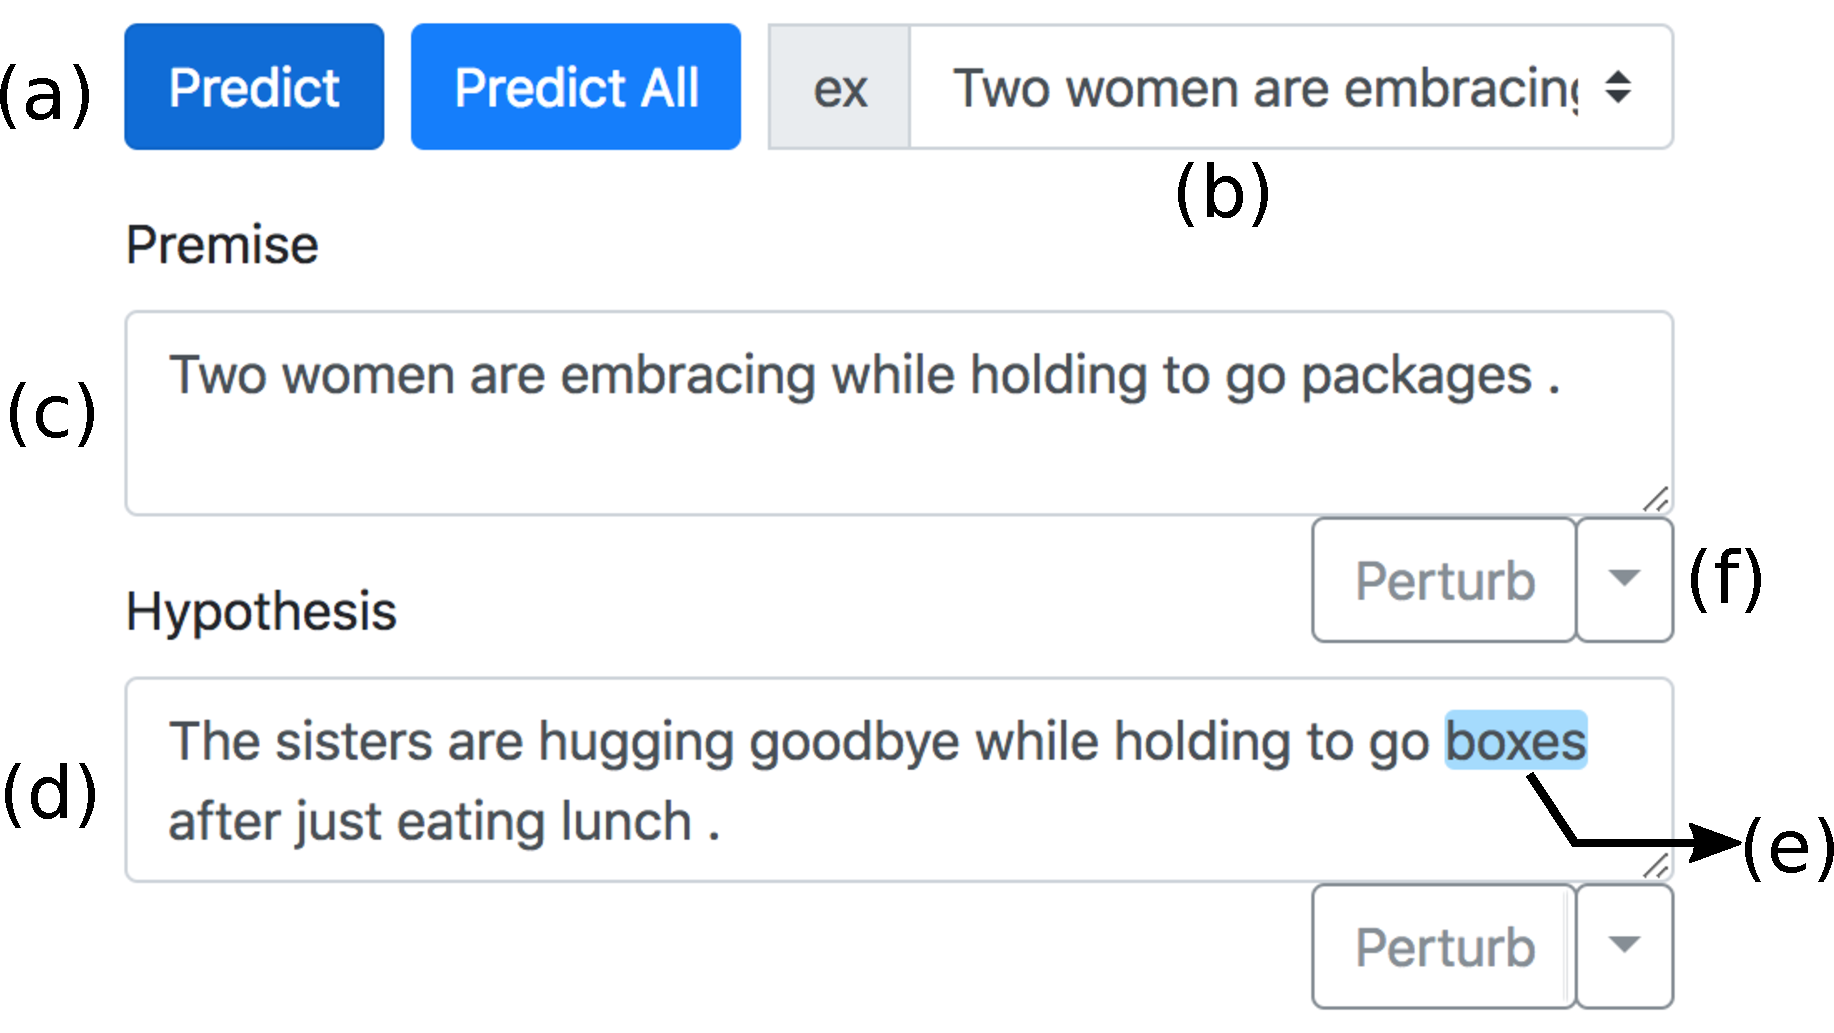
\includegraphics[width=0.95\linewidth]{sentenceView}
 \caption{
Sentence view shows the premise (c) and the hypothesis (d) sentence pair. The word that replaces the original text is highlight in blue, as illustrated in (e)
In (a), \emph{Predict} and \emph{Predict All}, each corresponds to predict the current displayed sentence pairs, or predict all combinations of perturbed premise and hypothesis.
In (b), previous explored original sentence are stored in the dropdown list that allow the user to revisit previous examined sentence.
 }
\label{fig:sentenceView}
\end{figure}

%\begin{itemize}
%\item Examine perturbed pair
%\item See which word is perturbed in a sentence
%\item Add to existing example collection
%\end{itemize}
